\documentclass[twocolumn]{IEEEtran}
\usepackage{url}
\usepackage{amsmath}
%\let\proof\relax \let\endproof\relax
\usepackage{amsthm}
\usepackage[linesnumbered,ruled]{algorithm2e}
\usepackage{verbatim}
\usepackage{graphicx}
\usepackage{subfigure}
\newtheorem{theorem}{Theorem}
\newtheorem*{theorem_nn}{Theorem}
\newtheorem{lemma}{Lemma}
\newtheorem{definition}{Definition}
\newtheorem{corollary}{Corollary}
\newtheorem{proposition}{Proposition}
\newtheorem{conjecture}{Conjecture}
\newtheorem{prob}{Problem}
\newtheorem{lemm}{Lemma}
\theoremstyle{definition}
\newtheorem{IP}{Integer Program}
\newtheorem{remark}{Remark}
\newtheorem{deff}{Definition}
\newtheorem{claim}{Claim}
\newtheorem{examp}{Example}
\newtheorem{prop}{Property}
\newtheorem{propp}{Proposition}
\newtheorem{assume}{Assumption}
\graphicspath{{figures/}}
\usepackage{amsmath}
\usepackage{mathrsfs}
\usepackage{amssymb}
\usepackage{booktabs}
\usepackage{changepage}
%\newcommand{\shrinkfig}{\vspace{-0.5cm}}
\DeclareMathOperator*{\argmax}{arg\,max}

\usepackage{tikz}
\usetikzlibrary{arrows}

\begin{document}

\section{Edge-clustering coefficients}
Let $G = (V, E)$ be an undirected, unweighted graph.
$N(u) = \{ w \in V : (u,w) \in E \}$.
\begin{definition}[Local clustering coefficient of an edge]
  Let $(u,v) \in E$. Then
    \[ c(u,v) = \frac{ | N(u) \cap N(v) | }{ | N(u) \cup N(v) \backslash \{u, v \} | }. \]
\end{definition}

This definition is similar to the one in \cite{}, which replaces
the denominator above with $\min \{ |N(u)| - 1, |N(v)| - 1\}$.

\subsection{Longer cycles}
\section{Edge-clustering in Multiplex networks}
Let $\mathscr{G} = ( G_\alpha = (V_\alpha, E_\alpha) )_{\alpha \in \Lambda} $ be a multiplex.
A vertex in the multiplex can be specified by a node-layer pair $(u, \alpha)$, where $u \in V_\alpha$
and $\alpha \in \Lambda$.
Consider an edge in layer $\gamma$, 
specified by $((u,v), \gamma)$, where $u,v \in V_\gamma$.
We consider triangles that include $((u,v), \gamma)$
and that have one edge in layer $\alpha$ and one in layer $\beta$,
for any $\alpha, \beta \in \Lambda$. These triangles
lead to a local clustering coefficient for $((u,v), \gamma )$ with
respect to the pair of layers $(\alpha, \beta)$.

For a node $v \in V_\lambda$,
let $N_\lambda (v)$ be the set of neighbors of $(v, \lambda)$ in layer
$\lambda$, for any $\lambda \in \Lambda$. That is,
\[ N_\lambda (v) = \{ w : (v,w) \in E_{\lambda} \}. \]
\begin{definition}[$(\alpha, \beta )$-local edge clustering coefficient] \label{def:ablecc}
  Let $\gamma \in \Lambda$, and let $e = (u,v) \in E_\gamma$. Then,
  \[ c_{\alpha,\beta}( e, \gamma ) = c_{\alpha,\beta}( (u,v), \gamma )  = \frac{ \left|N_{\alpha}(u) \cap N_{\beta}(v) \right| }{ \left| N_\alpha(u) \cup N_\beta(v) \backslash \{u, v\} \right|  }. \]
%w_{\alpha \beta \gamma}
\end{definition}
Definition \ref{def:ablecc} is illustrated in Fig. \ref{fig:ablecc}.
Notice that, in general, $c_{\alpha , \beta } ( e  ) \neq c_{ \beta, \alpha } ( e )$.
If $e = ((u,v), \gamma)$, and $\alpha = \beta = \gamma$, then $c_{\gamma, \gamma} ( e )$
reduces to the monoplex edge-clustering coefficient of $e$ in layer $\gamma$.
\begin{figure}
  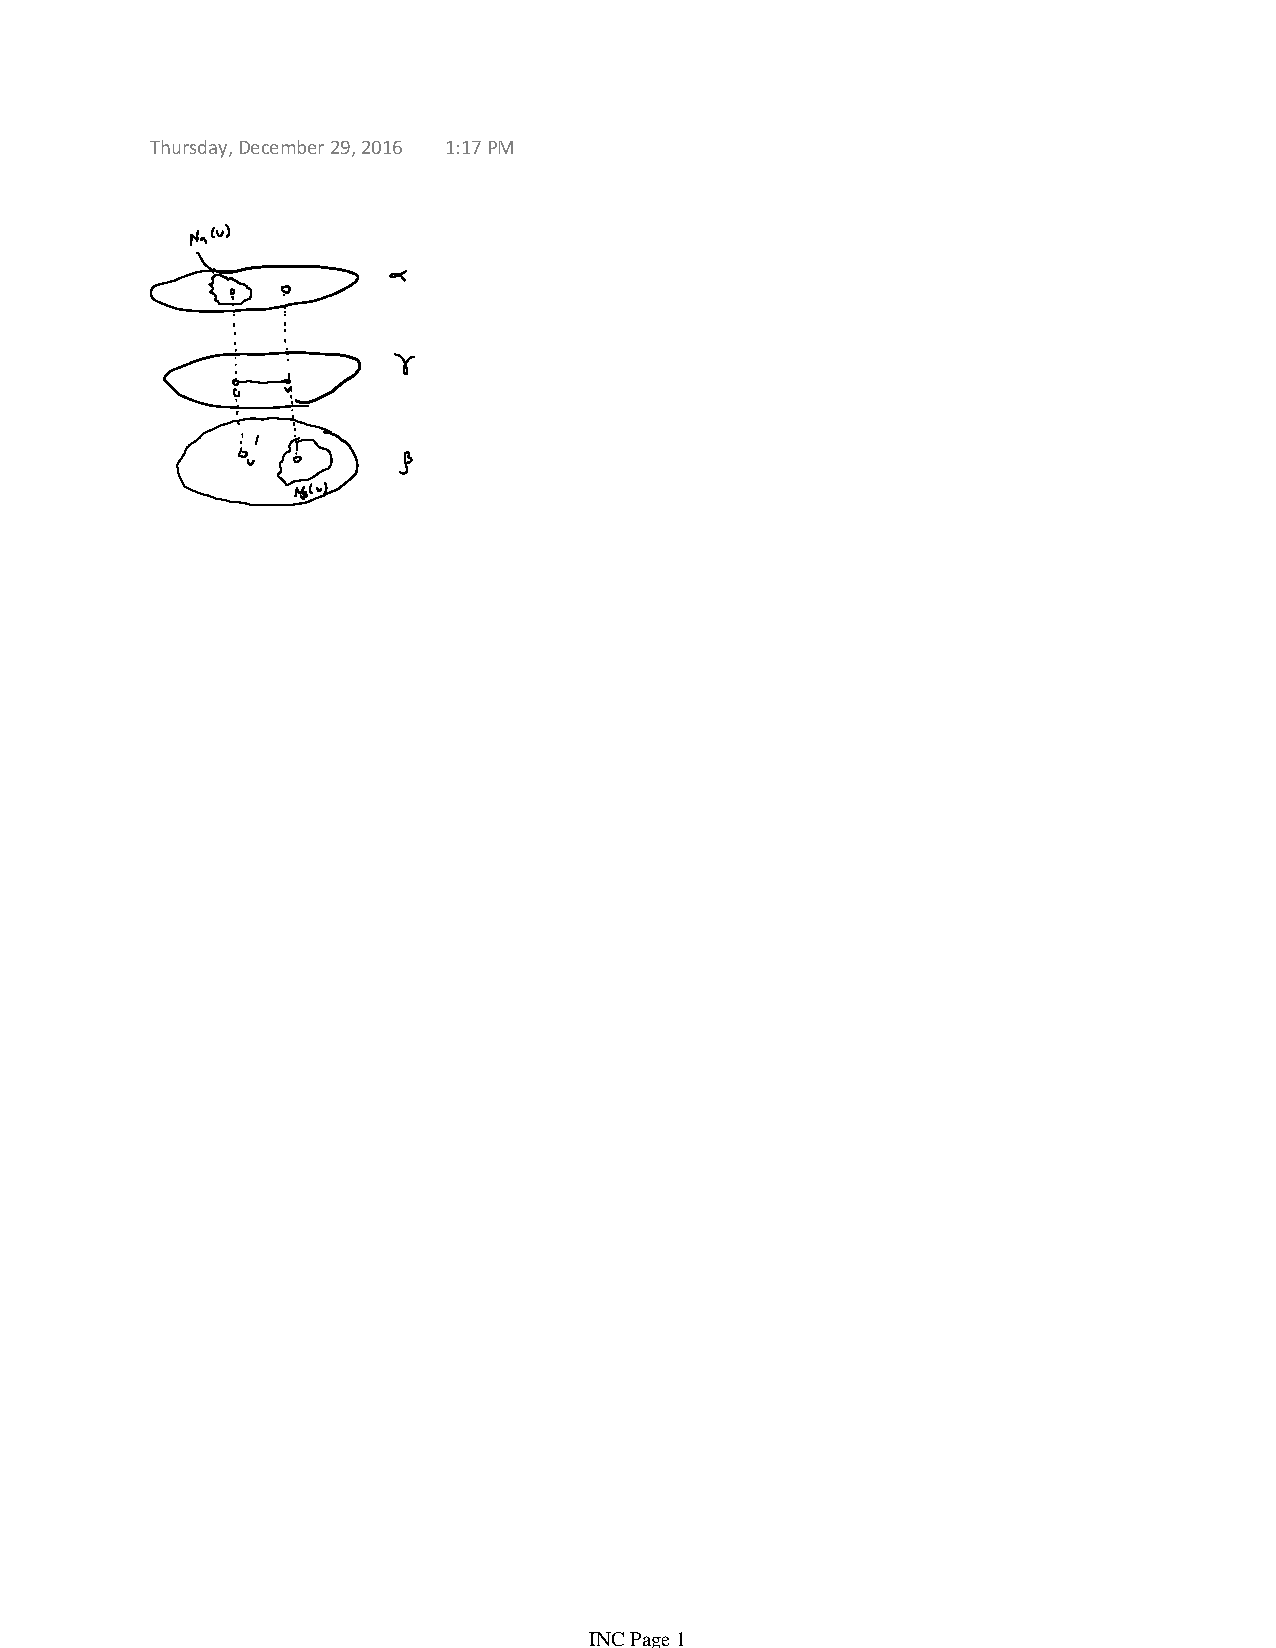
\includegraphics[scale=1.0]{fig1}
  \caption{ Illustration } \label{fig:ablecc}
\end{figure}
To obtain an aggregate measure over all layers for local clustering
of edge $e$, we propose the following method. Let
weight $W = \left( w_{\alpha \beta \gamma} \in [0,1] \right)_{\alpha, \beta, \gamma \in \Lambda}$.
$W$ quantifies the impact of layers $\alpha, \beta$ on layer $\gamma$.
Then, we define
\[ c( e, \gamma ) = \sum_{(\alpha, \beta) \in \Lambda^2} w_{\alpha \beta \gamma} c_{\alpha, \beta} ( e ), \]
and finally the local edge clustering coefficient of $e$:
\[ c( e ) = \frac{1}{ \left| \{ \gamma : e \in E_\gamma \} \right| } \sum_{ \gamma : e \in E_\gamma } c( e, \gamma ). \]

\section{Edge-clustering in Multilayer networks}
\end{document}
